

This chapter is dedicated to the fundamental concepts and current research in different areas related to this project: radiation effects on SRAM-FPGAs, soft-error, hard-error. Fault-injection, SEUs, Signatures, benchmarks for radation testing, and behavioral fault modeling. All of these topics are equally relevant for the purpose of this research that, ideally, places itself as an attractive research project.


%Most of the work done so far for soft-error analysis and evaluation is either on employing simulation framework, using fault emulation system on hardware, i.e., emulate faults on  FPGAs, and based on the efforts to find the analytical expression that represent the faulty behavior of the system

\section{Radiation Environment}


The electronics systems operate in the space are exposed to radiations. The first evident were observed in the sixties but it was difficult to separate soft-error from the other form of interference. The first evidence of malfunctions in electronic circuits embarked in spacecraft caused by the radiations reported in may 1979. In the outer space there are three main types of radiative sources that effects the Earth's atmospher.

\begin{itemize}

\item Galactic cosmic rays.

\item Radiation from the sun, i.e., solar wind and solar flares.

\item Earth's magnetic field, e.g., magnetospher and radiation belts.

\end{itemize}


\textbf{Cosmic Rays:} The origin of cosmic rays is hardly known. However, we have information about they are energetic particle spread throughout the galaxy including the solar system. This radiation comes from sources present in and out of our
galaxy. Interactions with interstellar matter, shock waves and 
electromagnetic fields accelerate this radiation. As a result, at the scale of our
solar system, it appears with an isotropic angular distribution and the particles are ionized. The sun is also the origin of some of these particles, but most of them come from the galactic sources known as galactic cosmic rays (GCR) wulf 22016.
Cosmic radiation was discovered by V. Hess in 1912 through measurements made from balloon probes. The cosmic rays constitute of 85\% of proton that is basically nuclei of hydrogen atom, 12\% are alpha particles that is helium nuclei, and the others are electrons and nuclei of heavier atoms. The energy of cosmic rays ranges from 1GeV to 108 TeV. lafebre.


\textbf{Radiation from the Sun:} The Sun alone accounts for 99.8\% of the total mass of the solar system, the remaining 0.2\% including planets, including the Earth. The sun is mainly composed of hydrogen (90%) and helium (8%). In the center of the Sun, thermonuclear fusion reactions convert hydrogen into helium. The energy produced on this occasion is emitted in the form of light,
of radiation and particles. The sun has two essential sources: feeding the terrestrial radiative environment: solar flares and solar winds. 

\textbf{Solar Flares:} The activity level of the sun is never constant but follows a cyclical variation that composed of active years followed by calm (no activity) years. The period of recent solar cycles has
varied between 9 and 13 years, with an average of about 11 years. The last cycle has ended around 2007 and since solar activity is growing again. The activity of solar cycles is frequently measured by the number of sunspots observed, but many
Solar processes show the same variation. Figure I-2 shows proton generated from solar events during five solar cycles. The curve shows the number of sunspots and vertical lines indicate the generation of solar protons. The first sunspot was observed in 1610 by Galileo while he devoted himself to the observation of the sun. The number of sunspots varies cyclically and most events
generating important proton influence appear during active solar years. During a solar cycle of 11 years, there are 4 years of low activity and 7 years of strong activity, punctuated by sporadic emissions of large particle fluxes, In this radiative context, there are two types of solar flares:
- Proton solar flares, lasting from a few hours to a few days, and
whose primary emission consists of protons of significant energy (up to
a few hundred MeV). The reference in this area is the August proton eruption 1972 visible in Figure I-2.
- Solar flares with heavy ions, whose main emission consists of heavy ions variable composition from one eruption to another, and whose duration is at most a few
hours. The reference in this field is the heavy ion eruption of September 1977.

\textbf{The solar wind:}
The solar corona causes the solar wind to dilute in space. The solar corona is the outer part of the Sun's atmosphere. It represents with the astronomical unit (1UA = 1.51$^{11}$ m). The solar wind fills the entire solar system and
interacts with the magnetic fields of the planets creating magnetospheric cavities. The
plasma density is of the order of 10$^{12}$ particles per cubic centimeter at the sun and falls to 10 particles per cubic centimeter at the Earth's orbit. This plasma is
primarily consisting of electrons, protons, and helium.


\textbf{The Earth's magnetic field}
The terrestrial magnetosphere is a natural cavity in the space environment in which the
Earth is relatively protected from outside influences. It is compressed on the side making
face to the Sun, and stretched to the other. It is a region of space dominated by the interaction between
the solar wind and the geomagnetic field (Figure I-4). However, at polar sides
the geomagnetic rigidity is reduced and therefore the particles from the
cosmic rays that have polar trajectories can penetrate to low
elevations. Satellites whose orbits have large inclination angles are therefore more
exposed to cosmic particles. The magnetospheric cavity resulting from the interaction of the solar wind with the field
geomagnetic is not static; it is subject to variations in the solar wind and the
interplanetary magnetic filed. The result is a complex dynamic at the origin of the magnetic storm events whose most spectacular manifestations are the aurora borealis.
and radio disturbances.

\textbf{Radiation Belts:}
Radiation belts commonly known as Van Allen Radiation belt constitute of charged particles trapped within the magnetosphere.
Discovered in 1958 by J.A Van Allen (Explorer I mission), these belts are located in the outside the Earth's atmosphere but still in the area of space influenced by the magnetic field of the Earth. The light charged particles (protons and electrons) named inner belt and the outer belt is formed by the energetic electrons, and the energies in between ten KeV to hundred KeV.

 

Van Allen belts count: 
\begin{itemize}

\item 2 electron belts centered at altitudes of 9,000 km and 60,000 km 
\item  1 proton belt at an altitude of 12000 km 


\end{itemize}
The dissymmetry of these belts is due to the deformation of the magnetosphere under the effect of solar wind and the inclination between the magnetic axis and the axis of earth rotation. 
The magnetic flux is very low and the proton fluxes change according to the altitude and
solar activity.


Based on the above information: we can conclude that many forms of radiations are interacting with the Earth's atmosphere. Ionized radiations make the case more severe for the microelectronics. These cosmic rays and solar particles continuously bombarding the Earth's and colliding with the atoms mainly nitrogen and oxygen which is 80\% and 20\% of the atmosphere respectively. These particles interact in two ways: either they lose some of their energy by ionization, or they may cause nuclear reactions thus forming a shower of
secondary particles (Figure I-8). The secondary particles generated are essentially:
neutrons, protons, electrons, muons, pions, photons (Figure I-9). 


Concerning radiation effects on electronics, the neutron particles are the most prominent. Neutrons are measurable at the altitude of 330 Km and their density increases until it reaches around 20 KM altitude. However, the density decreases below the 20 KM altitude and about 500 times lesser at ground level as compare to 20 KM altitude. For avionics the \textbf{neutrons} are the dominant particles.  Until 90's the neutrons with energy above 100 MeV were considered dangerous for electronics components. But due to the shrinking the transistor size, circuits are now become more sensitive to the low energies. Although the neutrons are non-ionized particles, they can hit different atoms, interact with the semiconductor generate ions that may produce faults.   

\subsection{Fault Caused by Cosmic Rays in Digital Circuits}


Ionizing particles can cause transient, permanent or destructive effects in the materials they pass through. They can therefore interact with embedded electronics and have critical consequences for the success of a space mission or avionics altitudes flights. Following the interaction, two types of effects emerge ---
single event effects (SEE) (caused by a single particle) and the total ionizing dose. In this research work we mainly focused on the SEE.


A Single Event Effect (SEE) results from a single energetic particle. When the particle strikes a sensitive node in a semi-conductor device, the ionization by the particle might produce a current pulse inside the device, which might cause soft or hard errors in the configurtaion memory of the device. Results in data corruption, transient disturbance, high current conditions (non-destructive and destructive
effects). If SEE cannot handle well cause unwanted functional interrupts or in worst case catastrophic failures. Commonly, SEEs include: single event upset (SEU), single event latch-up (SEL), single event burn-out (SEB), and single event transient (SET) etc as mentioned in Table~\ref{SEE-Summary}. 


\begin{table}
\caption{Single Event Effects Summary~\cite{manuzzato2010single}}
\centering
\label{SEE-Summary}
\scalebox{0.7}{

   \begin{tabular}{c|c|c}
         \toprule
    \hline
     
     Single Event Upset (SEU)                  & corruption of the information \\ & stored in a memory element            & Memories, latches in logic devices                                  \\ \hline
    
    Multiple Bit Upset (MBU)                  & several memory elements \\ & corrupted by a single strike                & Memories, latches in logic devices                                  \\ \hline
    Single Event Functional Interrupt (SEFI) & corruption of a data path      & Complex devices with built-in state       \\ \hline
    Single Hard Error (SHE)                   & unalterable change of state in\\ & a memory element                     & Memories, latches in logic devices                                 \\ \hline
    Single Event Transient (SET)              & Impulse response of certain\\ & amplitude and duration                  & Analog and Mixed Signal circuits                      \\ \hline
    Single Event Disturb (SED)                & Momentary corruption of the\\&information stored in a bit             & combinational logic, latches in logic devices                       \\ \hline
    Single Event Latchup (SEL)                & high-current conditions                                              & CMOS, BiCMOS devices                                                \\ \hline
    Single Event Snapback (SESB)              & high-current conditions                                              & N-channel MOSFET, SOI devices                                       \\ \hline
    Single Event Burnout (SEB)                & Destructive burnout due to\\ & high-current conditions                  & BJT Power MOSFET    \\ \hline
    Single Event Gate Rupture (SEGR)         & Rupture of gate dielectric due\\&to high electrical field\\ & conditions & Power MOSFETs \\ \hline
    
    \bottomrule
    
    \end{tabular}
    }
\end{table}



\subsection{Single Event Effects Mechanism}


When a particle passes through a semiconductor, it can directly or indirectly deposit charges in the silicon: a heavy ion deposits this charge linearly, it is why it is associated with a characteristic LET (linear energy transfer). This notion of deposit
charge is actually the translation of the generation of electron-hole pairs (Figure I-10a). Near the junction, these
pairs will first recombine (Figure I-10b) at the polarized reverse PN junction.  Then quickly diffusion principle will prevail (Figure I-10c). The duration of this
process is variable and can last from a few picoseconds to a hundred
nanoseconds.


\subsection{SEE Effects on FPGA}



FPGAs are complex reconfigurable devices that comprise a wide family of different resources. The basic structure of modern FPGAs includes interconnect resources, clock-management resources, configurable logic blocks (CLBs), input/output
blocks (IOBs), and embedded blocks such as digital signal processors (DSPs), general-purpose processors, high-speed IOBs, and memories. CLBs are used to perform simple
combinational and sequential logic. These blocks are typically formed of look-up tables
(LUTs), multiplexers, flip-flops, and carry logic. Programmable interconnect resources, such
as routing switches, allow interconnecting CLBs, IOBs and embedded blocks to implement multiple systems (Buell et al., 2007).
The logic and routing resources in an FPGA are controlled by the bits of a configuration memory, which may be based on either antifuse, flash, or SRAM technology. The
design flow of FPGA-based systems as shown in Figure~\ref{fig:fpga-struct} adapted from ~\cite{hauck2010reconfigurable} involves the creation of a bitstream to load into the
device.



\begin{figure}[tb!]
 \centering
  \captionsetup{justification=centering}    
   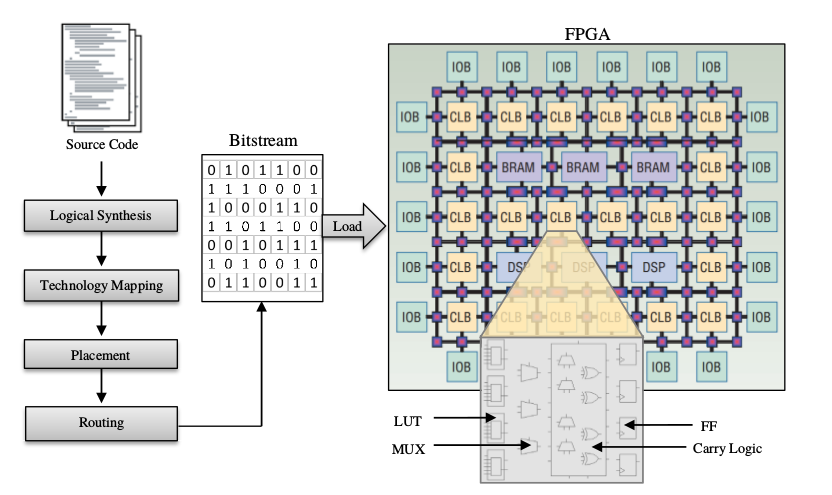
\includegraphics[scale=0.4]{figures/img/FPGA-structure.png}
   \caption{FPGA Structure and Design Flow}
\label{fig:fpga-struct}
\end{figure}




The process starts with the system design written
in a hardware description language (HDL), e.g., VHDL or Verilog. Next, the design is optimized and mapped into the FPGA’s available resources through logical synthesis,
technology mapping, placement, and routing. Finally, the generated bitstream downloaded into the device, and the device starts functioning according to the designer design.
Like any other semiconductor device, FPGAs are sensitive to radiation effects (due to neutron).
Mostly, these effects depend on the technology used to store the configuration data.
The foremost concern for SRAM-based FPGAs is
SEUs within the configuration memory, because the configuration memory controls all the operations e.g., data and control.
Upset configuration bits may change the logic and routing of the implemented system, as
shown in Figure~\ref{fig:seu}, leading to functional failures in an unpredictable way. In contradiction, the primary concern for anti-fuse and flash-based FPGAs is SETs and SEUs within user flip-flops
and block memories. However, the configuration memory blocks of anti-fuse and flash-based
FPGAs offer a relative immunity to SEEs, but these devices have lower logic capacity and
cannot be reprogrammed an unlimited number of times (flash-based) and anti-fuse only time programmable, making SRAM-based FPGAs more
suitable for complex systems requiring frequent reconfiguration and adaptation~\cite{quinn2015validation, violante2004simulation}. Errors produces in the FPGAs due to SEU can be classified into two different categories - errors affecting the logic blocks and errors affecting the routing~\ref{sterpone2006new}. For the logic block the SEU can produce the following errors~\ref{sterpone2006new}.

\begin{itemize}
\item LUT error: SEU modified the one bit of the LUT.

\item MUX erros: SEU changed the configuration of the MUX in logic block.

\item Flip-Flop error: SEU modified the configuration of a FF.

Routing resources are about the 80 percent of FPGA resources, SEE can create different phenomenas that modifies the different programmable Interconnect Points (PIPs)~\ref{sterpone2006new}.

\end{itemize}



\begin{figure}
 \centering
  \captionsetup{justification=centering}    
   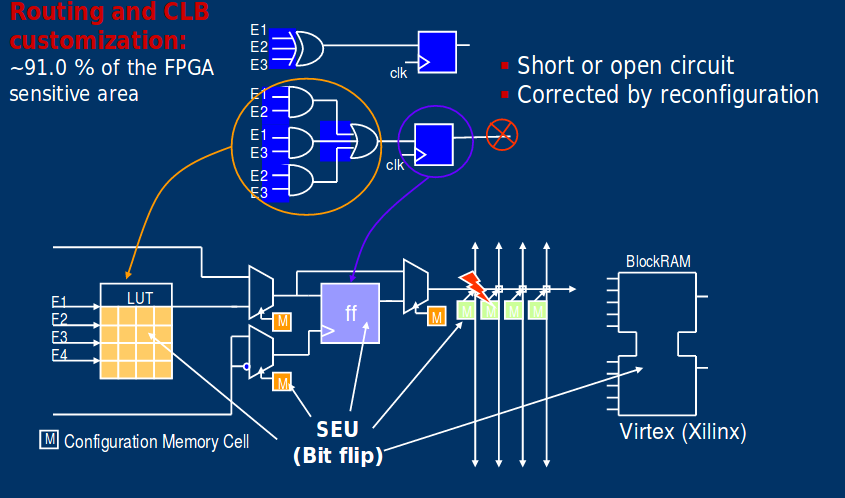
\includegraphics[scale=0.4]{figures/img/seu.png}
   \caption{Upset FPGA configuration bits may change the logic and routing.}
\label{fig:seu}
\end{figure}




%\subsection{Faults, and Failure}


\section{Design Verification by Fault Injection}




The second domain to understand in this project is designing, testing and verification by fault injection. As we discussed before, SRAM-based FPGAs are particularly sensitive to SEUs. The configuration memory is the most sensitive part. By changing the configuration memory, may affect the overall functionality of the system. The work done so far to study the SEU effects on FPGAs, combines the emulation, simulation, and radiation testing

\subsection{Emulation}

The purpose of fault emulation to reproduce as closely as possible radiation based results, evaluate the criticality of FPGA resources, analyze the impact of flipping the critical bits, find the faulty response of the circuit by flipping the bits and find techniques that help to reduce the emulation time. Several works have been done so far deals with the analysis of SEU effects on FPGAs. The emulation of SEUs in an FPGA is done by flipping the bit in the configuration memory. 

The work presented in ~\cite{hobeika2014multi} provide an emulation platform for the signature generation. This work is focused on the identification of the emulation zone,  fault list generation, SEU emulation, result Analysis. The purpose of their work is to investigate the sensitivity of SRAM-based FPGAs devices not only for the simulation-based approach but also used emulation and radiation testing for evaluating the effects of SEUs. In this paper they also provide the results for the radiation based signature and simulation based signature. They showed that simulation and emulation based signatures could contain the same error values as obtained with radiation but their probability of occurrence could significantly different. The arithmetic signature for TRIUMF to emulation is 85.3 % for adder and 84.8% for the multiplier. Similarly, the matching with the simulation of adder and multiplier with TRIUMF is 84.8 % and 100 % respectively.

The work presented in~\ref{souari2015optimization, souari2016towards} deals about the fault injection into the FPGA configuration memory based on the sensitivity of the bits by considering that the 'bits-at-one' are more sensitive to the "bits-at-zeros". The Emulation setup presented in this paper adopted the approach for the estimation by fault injection based on the sensitivity. Authors proposed the method in which fault are injected based on the specific bits configurations defined according to their contents and the type of FPGA resources.



They have developed a methodology to extract the list of configuration bit addresses of the design LUTs based on the .ebc file of the design.  For the identification of an emulation zone, they used the concept of the essential bits which can be extracted by the Xilinx BitGen command.

The work presented in~\cite{quinn2015using} described the benchmark that can be used for the reliability and radiation effects study on FPGAs and microprocessors. 

An accelerated fault injection technique is presented in~\ref{di2014fault} bassed on the design essential bits provided by the \textit{bitgen} command of Xilinx ISE tool. Similarly, there are few other techniques are availble for the fault emulation based on the random fault injection, two board FPGA and single FPGA~\ref{faure2005single}.


The work  proposed in the~\cite{hobeika2013flight} described a completed automated methodology to emulate SEUs on an FPGA efficiently. The authors used the reconfigurable flight control system based on a reference adaptive control model. 
In this work, 253227 bits are identified as the total essential bits among them, 57464 belongs to the interested essential bits. The step is used to minimize the time because an FPGA device contains millions of configurable bits, emulating a bit flip for every cell would be time-consuming. BitGen gives only the essential bits; that
considered critical bits.  

The difference between the work presented in~\cite{hobeika2014multi} and~\cite{hobeika2013flight} is that; in~\cite{hobeika2013flight} the authors used the flight control system that is based on a linear plant model. Whereas, in~\cite{hobeika2014multi}the emulation is performed on the circuits (adder and multiplier). 



%\begin{itemize}
%
%\item   {Classification of the configuration bits into subsets.
%        a.  Bits set to 1/0 of LUT.
%        b. Bits set to 1/0 configuring other than LUT.
%        c. Bits set to 1/0 configuring other resources not identified as  potentially critical by bitgen.}
%        
%        
%\item  {Estimating the number of critical bits of the set by randomly injecting faults in the bits of each set. This method helps to find the most critical zones of the FPGA.}
%
%\item {Prioritized the fault injection in the identified (step-2) most critical zones.
%These classification steps are done with the help of EBC and EBD files provided by the bitgen. The experimental results presented in [5] evaluated the SEU sensitiveness as well as bitgen efficiency. The results are evaluated between random fault injection with different prioritized bit subsets.  The first observation authors concluded - the bitgen did not accurately identify all the critical bits meaning the bitgen limitations. Second authors did the prioritizing the most sensitive subset. It would involve exhaustive fault injection. The authors used fault injection to get an estimated number of critical bits as well as the related estimation error. They used the term critical bit error estimate (CBEE). The authors claimed the CBEE observed for the random approach is higher than the observed under the bits subsets.  The ratio of observed critical bits (ROCB) observed for the random injection is far less than the different bits subsets.}



%\end{itemize}

\subsection{Simulation}

Simulation based testing are low cost and flexible but it is difficult to get the accurate results from the simulation based testing. For simulation based testing the work presented in the~\cite{violante2004simulation} described a approach for fault injection based on the simulation during early design phase when the hardware system is not ready. The work presented in~\ref{robache2013methodology} demonstrates how faulty behavior signatures allow building high-level models, i.e., high-level faulty model, e.g., fault model in MATLAB Simulink, that reflects the faulty behavior of a combinational circuit represented at gate-level. The fault injection tool that is used named - LIFTING.  The purpose of this tool is to study the effects of different types of faults on a circuit at gate-level. The tool used the stuck-at 0 and 1 are injected in each node of the design. The LIFTING is a simulation-based gate-level fault injection tool that used the circuit netlist file, e.g.  *.v file, input test vectors, and fault parameters as inputs produced two output files. The one is the golden report and the second consist of fault injection report. These two outputs are used to generate the signatures.  The signature represents the compressed faulty behavior of the circuit. The signatures consist of arrays of errors and their probabilities of occurrence. The signatures are either arithmetic or logic.  The third step is to make a high-level model that corresponds the low-level circuit. The work presented in this paper helps to make a faulty block with Simulink that reads a signature and generates errors according to the distribution.

\subsection{Radiation Testing}
Radiation testing is an expensive approach and requires a state-of-the-art facility. The work presented in~\cite{hobeika2014multi} described the effects of radiations on a circuit modeled at a low- level and then abstract it to a  higher level. In this work the also compared the results which are expressed as signatures of fault simulation, emulation, and radiation. They  want to capture and regenerate the faulty behavior occur due to SEUs early in the design process. Their hardware setup consists of two Artix-7 board. Board A used as a reference and board- B is subjected to radiations. The board-A is not bombarded, and it hosted the counters, reference design error detection and signature computation, memories to store signatures and communication controller. A total 20 runs performed on the adder and 14 on the multipliers. Arithmetic errors for both approached DSP and LUT are observed (151 vs. 291 for DSP). This is due to DSP strategy; SEUs can add registers in the data path, leading to the sequential type of errors. The authors in this work compare the results from the fault simulation, fault emulation, and radiation testing. 



The work presented in~\cite{dsilva2015neutron} used the Flash-based FPGA under neutron beam to observed the SEE in avionics applications. They observed that the failure in time rate for flip-flops, SRAM cell, PLL are resonably low. They proposed that the FFs can be hardened by the TMR. 

In~\cite{maillard2015neutron} authors tested the UltraScale Kintex FPGA under neutron and proton beam. They examined the single event upset response of the FPGA. They presented the result in terms of failure in time calculation. They observed that  there are 0.1\% are uncorrectable events. 


The work presented in~\cite{quinn2015using} did the radaition testing in the Los Almos Neutron Science Center (LANSCE). The results are provided for the micro-controller, ARM cores, GPUs, and FPGAs. The B13 from ITC99~\cite{ITC} is used under the hardware benchmark suite; Virtex- 5 is used as a hardware platform. They also provide the result for the mitigation. For mitigation, they used X-TMR and VERI-Place. The failure in time (FIT) are decreased under mitigation, but the overhead is increased (circuit area increased).

\textbf{Hardware Benchmark Testing}
For the hardware radiation testing the authors used the B13 from the ITC’99 benchmark suite. The circuit is too small so it can be replicated 30 times, the implementation is done on the Virtex-5. Both unmitigated and mitigated version are tested. The results for FPGA radiation reports SDCs from the mitigated circuits normalized to the SDCs from the unmitigated circuits. Mitigated circuits are likely to fail at three times the rate of the unmitigated circuit, because of the increased size of the circuit from the mitigation process. The mitigated circuit cross-section is three times larger than an unmitigated circuit when SEUs accumulate. The authors conclude; the VERI-place mitigated circuits perform better than the X-TMR mitigated circuits.

\textbf{Software Benchmark Testing}
Software benchmark radiation testing is done on the flash-based microcontroller,  a ferroelectric-memory-based microcontroller, two ARMs, and GPUs. These components are tested with both mitigated and unmitigated codes. The results reported in the paper for two different microcontroller and two ARMs cores. For microprocessors: these microprocessors have very small SRAM the FITs are very small. In some cases, there is no error from the code during many days of testing. They also implemented the matrix multiplication, FFT, and Hotspot on NVIDIA K20 GPU and applied mitigation methods (ECC, ABFT, and DWC).  The purpose is to see the effect of overhead by applying the mitigation technique; the overhead has been increased as compared it with the unhardened configuration.










%\subsection{Benchmark for Radiation Testing}
%The suitable selection of the benchmark for the radiation testing of microprocessor and FPGAs is a recently topic of ongoing research. The benchmarks are used to evaluate the performance under different architectures, technology, and compiler. There is no such standard benchmark employed to study microprocessor and FPGAs under the effects of radiations; make it difficult to assess the changes in fabrication technology, architecture, and circuitry. The work presented in~\cite{quinn2015using}described the software and hardware benchmark under the neutron test data. The unavailability of the such a benchmark for testing because radiation hardness assurance techniques are applied only to circuit layouts or manufacturing process. There is no standard test circuits available, researcher, used flip-flop or D-latches to compare their results. In recent years, radiation effects community shown interest to develop a standard set of circuits that include complex and realistic algorithms and can be adapted to different FPGAs.  Currently, without standard benchmark researcher used the following approach for testing:
%
%\begin{itemize}
%
%
%\item Homemade Design.
%\item Circuits from Opencore.
%\item Proprietary designs.
%\end{itemize}
%
%
%The problem with this approach as no two organizations used the same set of codes or circuits, difficult to make the comparison. There is a need for collaboration to make a suitable set of benchmark for reliability application and study the effects of radiation under the same conditions. The criteria used to set a standard benchmark including:
%
%Repeatability of benchmark tests.
%A representative of deployed computing workload.
%Availability of fixed input vectors.
%Cross-platform implementation.
%The ability to repeat test itself is an important part of the standardized testing. By repeating the algorithms, the input test vector, the compilation, the synthesis setting help researchers to have the enough information. It is necessary to provide a wide variety of realistic algorithms so that the system can be tested as likely to the realistic application. Defining the input test vector is an essential step because many hardware errors can be observed under the specific set of the test vector. It is an open question which input test vector should be adopted, under the specific set of criteria. Finally, the implementation of the algorithms in portable languages help to use the same set of codes on the different platform. For example, assembly language for the microprocessors limit the ability to compare and port codes on the different platform. But the hardware benchmark developed in VHDL can ease the problem; the same circuit can be ported to any FPGA.
%
%\textbf{FPGA Radiation Benchmark}
%
%The FPGA benchmark mentioned in this paper is ITC'99 which is well defined ATPG benchmark. This benchmark meets all the requirements, e.g., realistic algorithms, input vectors, scalability, and portability. The circuits are implemented in the HDL so that it can be ported to different FPGAs. The first 15 circuits from the ITC'99 are adopted for the benchmark as shown in Table I.

%\textbf{Software Radiation Benchmark}
%
%The software radiation benchmark is harder to design than the FPGA radiation benchmark. The development of the standard set of algorithm that can be ported on different architectures would be a challenging task e.g., porting an algorithm to 16-bit microcontroller to GPU. The authors are interested in the software benchmark where the computational load can be divided into the parallel processes or run on a single core. The commonly used software benchmark comprises of fast fourier transform, matrix multiplication and quick-sort algorithm as they are commonly used in many applications and useful for the evaluating the reliability of parallel processors. The software benchmark comprises the following code.
%
%\begin{itemize}
%\item AES-128;
%\item Cache test;
%\item FFT;
%\item Hotspot;
%\item HPCCG;
%\item Matrix Multiply;
%\item Quicksort
%\end{itemize}










%\section{Fault-detection, mitigation and correction in the FPGA }


%The impact of SEUs on SRAM FPGA devices has been studied in~\cite{bellato2004evaluating}. Many  techniques  have  been  proposed to provide highly reliable FPGA devices, e.g. radiation-hardened FPGAs~\cite{rockett2007radiation}, in-order to lower the effect of radiation-induced SEUs. However, radiation-hardened  SRAM  FPGAs  typically have  a  low  density, and  they  only  may  lower  the  probability of SEUs to occur but  not  completely avoid  them. Therefore, non radiation-hardened FPGAs, like the  Xilinx Kintex-7, are evaluated under a harsh radiation  environment~\cite{wirthlin2014soft}. Even on radiation-hardened FPGAs, the SEU rate in a low-earth orbit flight experiment can be up to 16 events per day~\cite{quinn2012orbit}. A wide  variety  of  SEU  fault  mitigation  techniques  for SRAM-based  FPGAs  have  been  proposed  during  the  past years. These techniques can be categorized into module redundancy techniques such as triple modular redundancy (TMR)~\cite{lyons1962use} and techniques that use scrubbing of the FPGA configuration memory~\cite{heiner2009fpga}. Also the combination of  both techniques has been shown to be able to increase the reliability of FPGA modules significantly ~\cite{ostler2009sram}. FPGA-based TMR approaches replicate a given module which shall be protected either statically or dynamically~\cite{angermeier2011runtime}. The different granularities of voted replicas  are evaluated in~\cite{bolchini2007tmr}. However, no upset rates and consequential no reliability figures are provided. Nevertheless, TMR techniques are  known to often cause an excessive and unacceptable overhead in terms of power  consumption and area. Since the intensity of a cosmic rays is not constant but may vary over several magnitudes depending on the solar activity, a worst-case radiation protection is far too expensive in most cases. A self-adaptive system is proposed in~\cite{glein2014self}, which monitors the current SEU rate and exploits the opportunity of partial reconfiguration of FPGAs to implement redundancy such as TMR on demand. 

%Memory scrubbing is a well-known correction technique for the configuration memory of SRAM-based FPGAs. It consists on re-writing the configuration memory after the FPGA is configured to restore its original content. It is often a transparent operation for the running application. This is possible because modern FPGAs offer a dynamic partial reconfiguration (DPR) feature. The circuit that enables the scrubbing is commonly named scrubber. Additionally, readback is the process of reading the configuration memory of the FPGA after it is configured. Both processes (readback and scrubbing) can be used to implement different scrubbing methodologies as shown in~\cite{herrera2013design}. Scrubbing can be implemented using an internal or external interface as shown in~\cite{berg2008effectiveness}. When external interface is used, the scrubbing logic is implemented outside the FPGA. In the case of Xilinx FPGAs several external interfaces are available; however, the Select MAP interface has the highest data throughput. On the other hand, there is only one internal interface named ICAP~\cite{xilinx}. This internal interface can be accessed from the reconfigurable logic of the FPGA and it is a replica of the Select MAP interface. Also scrubbers can be implemented in software or hardware. The scrubbing process can be implemented using a microprocessor with the advantage of a high flexibility to implement different complex scrubbing methodologies but with lower configuration speeds and lower energy efficiency.



\section{Fault Models}


The last domain of this work is related to the fault models, and fault analysis. We further divided this into three different categories and provide a related work on each domain separately. The most of the research work has been done is related to the transient fault analysis, soft error rate (SER) analysis and error prediction, failure-in-time calculations all these research done on the different abstraction levels.



\subsection{Behavioral Domain:}


In~\cite{chen2017fault} authors proposed the fault propagation process between the different subsystem of the
main system, combined with the finite state machine. This work is based on the FSM and fault propagation model. 

In~\cite{svenningsson2010model}, authors presented the idea that how model-based fault injection can be utilized to
simulate the effect of hardware related faults in embedded systems. Model level and hardware level
fault behavior comparison is presented.

In~\cite{hayne1999behavioral},  they proposed two tools, which facilitate the fault simulation of behavioral
models, described using VHDL. The tool is the Behavioral Fault Mapper (BFM). The BFM algorithm
accepts a fault-free VHDL model of the design (combinational circuit) and a fault list of N faults from
which it produces N faulty models. The assumed 8 different fault models, e.g., Stuck-Then, Stuck-Else,
Assignment Control, Dead Process, Dead Clause, Micro-operation, Local Stuck-data, Global Stuck-data. 

In~\cite{kapare2016automated}  they proposed a methodology to estimate the output quality of approximate
sequential circuits (faulty circuits) based on finding the analytical expressions for predicting
approximation errors from statistical data gathered from performing limited characterization of the
approximate circuits (faulty circuits). They proposed a methodology for estimating/predicting the output
quality of a faulty circuit. They want to accurately predict the error behavior. 

In~\cite{mirzadeh2014modeling} In this work, author proposed a fault behaviour model developed with a neural network
concept in a novel way. The neural networks (NNs) structure was used to synthesize the faulty output of a
circuit at a high-level of abstraction. All the strategies that were proposed in this research have novelty;
and effort is exercised to find an appropriate structure for the neural network. The idea is good to make a model with NNs. But it underestimate the power of NNs for
smaller circuits.


In~\cite{janschek2017errorsim} authors proposed the high-level fault behavior mode. This work  used for the error propagation analysis. The tool have the ability to simulate different fault-models, e.g., offset, stuck-at-fault, noise, delay, package drop, and bit-flip. 

In~\cite{hobeika2013flight} authors presented the new fault model that can be used by the designer at an earlier stage in the design process. In this work, they used the adaptive control model and did the SEU emulation on it. They found the new fault model, e.g., Control amplification, Sign Inversion, etc.

The work presented in~\cite{thibeault2013library} based on the C/C++ description of an application. They used the technique to convert the circuit into control and data flow graph (CDFG) file, then used the resource estimation tool, to find the resources required to implement an application on an FPGA.

The limitation of this work is the resources utilization tool for different FPGA. You need to modify the resource utilization for each new FPGA device. Moreover, this work is based on the .ncd file of the circuit provided by the Xilinx ISE tool, which is no more available for the newer FPGAs. 

The work presented at the behavioral level did not have the insight information of the how fault effect the hardware at the circuit level. For example, in~\cite{janschek2017errorsim} the supposed the fault distribution are normal, exponential, Poisson, Weibull. The methodology we present in this thesis based on the fault emulation at the circuit-level and abstract it to the high-level. So, in this case, we will get the information not only how the model works at the high-level but also get the real-time information about the fault behavior at the low-level.


\subsection{Transformation Domain}


The transformation of the circuit into their respective tools is costly procedure and assume alot of assumptions, e.g., fault assumption to cause error in the expression or node.



The work presented in~\cite{ubar2014modeling} is based on the Simulation, transformed the circuit into their required tool format, then they
insert the fault on different nodes and calculate the SER. 

In~\cite{brkic2014symbolic} the key idea behind this paper presented a symbolic analysis method for unreliable logic
gates. 

In~\cite{chan2013statistical} authors addressed the estimating output quality of a faulty hardware circuit by pre-
characterizing the relationship between Error metric behavior and characteristics of approximate
hardware circuits. These values are stored in lookup tables which are used to retrieve Error metric
composition for a given approximate hardware module and then compose error metrics for output
quality using regression-based models. This approach also takes into consideration the input
distributions of the faulty circuit. 


Modeling the probabilistic behavior of the Finite State Machine, calculating the steady state
behaviour of the circuit and used for estimating the switching activity of the circuit for the purpose of
power evaluation presented in~\cite{hachtel1996markovian}. They showed how steady-state probabilities of very large FSM’s can be computed by
symbolic ADD-based algorithms.


In~\cite{shazli2011high}, Soft Error Rate (SER) computation problem is modeled as a Boolean
Satisfiability (SAT) problem and SAT solvers are used to compute SER for combinational and
sequential circuits. They used an automated flow to convert combinational and sequential behavioral
descriptions into equivalent SAT instances. The use of Boolean Satisfiability (SAT) approaches, to
model soft errors in early design stages presented.



In~\cite{miskov2007mars}, the symbolic framework based on Binary Decision Diagram (BDD) / Algebraic Decision
Diagram (ADD) to analysis sequential reliability is presented in this paper. They calculate how much the
gate output is suspected of an error. The MES is calculated at the electrical (transistor) level regarding
the duty cycle, signal amplitude (voltage), and the gate error probability of individual gates associated
with different input probabilities. 




The limitation of working in this domain and make the model of the faulty behavior is to convert the design into respective tool, e.g., BDD/ADD, many assumptions, and simulations only. Need to drive the mathematical expressions for the fault model,  also need to assume the fault in the design, plus its too hard for complex circuits


\subsection{Circuit Level}


In~\cite{li2016monte} authors presented a  Monte Carlo technique for the soft error analysis of the sequential
circuits. They perform the logic simulation for latch-level error propagation to estimate the SEUs. This work is mainly focused on the SEUs convergence means after how many clock cycles the circuit becomes fault free.
They insert the fault into the simulator and observe it to the output. Apply the Monte Carol technique
to find the number of samples and the time for the estimation of the error
  
  

  The key idea behind In~\cite{ebrahimi2015comprehensive} is to present the result for SER analysis on an embedded
processor. There platform employs a combination of models at device level, gate level error
propagation and at architectural level. They used the
processor core and drive all the results via simulation of this core under the assumption of the fault. While using processor core under the radiations the primarily concerns is for the cache memory instead
of the core itself.


this technique  used in~\cite{ranjan2014aslan} is to estimate the output quality of a faulty circuit which uses the concept
of unrolling the circuit with each clock cycle and compares this faulty unrolled circuit with the original circuit
using a quality evaluation circuit and generates some vectors, which indicate the quality of the circuit
at that cycle. Unless the quality constraints are satisfied. The faulty circuit is unrolled every cycle with incremental improvements in each cycle. Thus,
if the desired output quality is high, the cost of unrolling and analyzing error metric also increases
substantially.

In~\cite{yu2010scalable}, authors developed novel and efficient ways to sample logic circuit behavior,
model the impact of soft errors, and estimate the circuit reliability. Their method was described that
used the probabilistic transfer matrices to calculate signal and error probability distributions in the
sequential circuits at the logic level. This work is mainly focused on finding the signal probabilities at the gate level. To do so
they partition the combinational part of the sequential circuit, and then find the probabilities of each
individual gates.


In~\cite{miskov2007mars},  they estimate the likelihood that a SET in a sequential circuit will lead to errors
in clock cycles following the particle hit, and find after the hit (which is an assumption) how many clock
cycles needs to get the SER below the threshold level. The main idea was to allow for symbolic modelingand efficient estimation of the susceptibility of a sequential circuit to soft errors. A symbolic modeling
methodology for efficient estimation of the soft error susceptibility of a sequential circuit.
Limitation: They solved the problem with the analytical approach. Almost similar to the previous work.~\cite{miskov2007mars},~\cite{miskov2008modeling}. There main concern after particle hit (in experiment they did not performed this) how many
clock cycles will it take to get SER decrease.




In~\cite{lingasubramanian2010probabilistic}, authors calculated the maximum error in digital logic circuits and the respective
worst-case input pattern, through maximum a posteriori hypothesis, using a Shenoy-Shafer algorithm.
They showed the importance of handling maximum error behavior for achieving fault tolerant
computing machines. They studied the circuit-specific error bounds for fault-tolerant computing. This work is mainly focused on finding the signal probabilities; convert the signal
probabilities into angles. Use conditional error model, which is not the case in real-time testing.
Simulation and assumption work. They calculated the average output error in sequential circuits and
studied the transient error behavior across different time instances, using a dynamic time evolving
probabilistic error model.

In~\cite{miskov2008modeling}, Markov chain for the steady-state behavior of the sequential circuits, Symbolic framework
based on the BDD/ADD is presented. They did the Single Error Rate (SER) evaluation, purposed to do
for the gate sizing, find the gate size that has the highest soft error impact based on this recommend
different gate size for the transistor technology. 
 




In~\cite{das2007monitoring}, Error Monitoring scheme to detect the Transient Error. The idea presented in this work has a worth to compute the error for each stage
independently. But they didn't provide they experimental setup details, no details for the how the fault
occurs in their system.

In~\cite{asadi2005soft}, they provide the multicycle analytical framework to analyze the multi-cycle error
propagation. The major limitation to their work is the measuring unit the used in their work “mean time
to manifest error.” The common terminology for this kind of work is SER. This is the simulation work,
with the assumption that the fault will occur in the flip-flop and proceed to other flip-flop. They did not
consider the fault occurs in the combinational logic of the sequential circuit.

In~\cite{miskov2010multiple}, the key idea presented in this paper is to analysis the susceptibility of the circuits outputs
errors originating from the single or multiple fault transients faults. They are keener to find the part of
the circuit that has the highest error generating probability.





The work done in this domain use only simulation, assume fault occurs, suppose the glitch size, and assign the
probabilities in the HSPICE simulator. Authors make the model of the faulty circuit by supposing it gets
fault make a model with Markov chain, ADD/BDD and then compare it with the simulation using the
HSPICE. They also assume that an error occurs only in the first clock cycle of a w-cycle simulation with
no new errors occurring in subsequent cycles. It has difficulty simulating circuits over many cycles
because of the way it employs the time-frame technique. Moreover, fault can occur in combinational part of the sequential circuit as well. The circuit size and the number of primary
inputs and outputs grow linearly with the number of simulated cycles, and memory usage becomes
unmanageable after a few simulated cycles. Another source of inaccuracy in fault analysis at this level is it
assumes an error occurs only in the first clock cycle of a w-cycle simulation, and no new errors arrive in
subsequent cycles.












\label{related}
\section{Relation to State-of-the-Art}
The work done so far [1, 2, 3, 4, and 5] evaluated and quantified the SEU effects by performing simulation, emulation, and radiation on an SRAM-based FPGA. Implemented a design, observed its faulty behavior in the presence of SEU and extracted the corresponding fault model. Presented an automated methodology to efficiently used the SEU controller. Discussed the fault injection on the specific subsets rather than random and discussed the selection of the suitable benchmark for FPGA and microprocessor radiations. 




%%% Local Variables:
%%% mode: latex
%%% TeX-master: "../Document"
%%% End:
